\renewcommand{\thechapter}{HS}
\chapter*{Homework Solutions}
\addtocounter{chapter}{1} % Manually increment the chapter counter
\markboth{\sffamily\normalsize\bfseries Homework Solutions}{} % Set the chapter header
\addcontentsline{toc}{chapter}{\textcolor{ocre}{Homework Solutions}}
\setcounter{section}{0}
\vspace{-0.3in}
\begin{tcolorbox}
    I encourage you to give each of the homework sets an honest attempt before looking at the solutions, you will get much more out of reading the solutions if you have first spent time carefully thinking about the problems on your own!
\end{tcolorbox}
\vspace{-0.2in}
\section{Homework \#1 Solutions}

\begin{enumerate}
    \item We are given the relation $\sim$ on $\R$:  
          \[
          \forall \ r,s \in \R, \quad r \sim s \iff r - s \in \Z
          \]
          and we are to show that $\sim$ is an equivalence relation.

          \textit{Proof:}  
          \begin{enumerate}
              \item \textbf{Reflexivity:} Take $r \in \R$. Then $r - r = 0$, and $0$ is an integer, so $r \sim r$.
              \item \textbf{Symmetry:} Assume $r \sim s$. Then $r - s$ is an integer.  
              Its ``opposite'' $-(r - s)$ is also an integer, so $s - r \in \Z$ and we have $s \sim r$.
              \item \textbf{Transitivity:} Assume $r \sim s$ and $s \sim t$.  
              Then $r - s \in \Z$ and $s - t \in \Z$. The sum of two integers is again an integer, so  
              \[
              (r - s) + (s - t) \in \Z
              \]
              so $r - t \in \Z$, so $r \sim t$. $\blacksquare$
          \end{enumerate}

    \item \begin{enumerate}
              \item The equivalence class of $\pi$ is given by:
                    \[
                    \text{cl}(\pi) = \{ r \in \R \mid r \sim \pi \}
                    \]
                    which means:
                    \begin{align*}
                        \text{cl}(\pi) &= \{ r \in \R \mid r - \pi \text{ is an integer} \} \\
                        &= \{ r \in \R \mid r = ( \text{an integer} ) + \pi \} \\
                        &= \{ n + \pi \mid n \in \Z \} = \{ \dots, -1+\pi, \pi, 1+\pi, 2+\pi, \dots \}
                    \end{align*}
                    This is usually expressed as $\pi + \Z$.
                    \begin{center}
                        \hspace{-0.1in}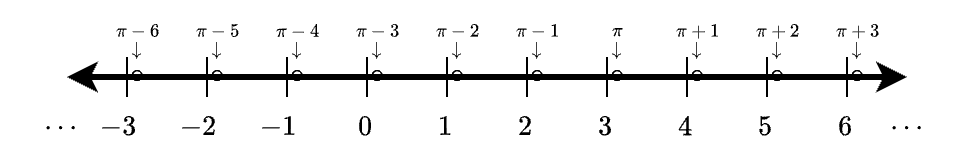
\includegraphics[width=0.85\textwidth]{Figures/EquivClassOfPiNumberLine.png}
                    \end{center}

              \item For any $s \in \R$, we can similarly find $\text{cl}(s)$ by substituting $s$ for $\pi$, so:
                    \[
                    \text{cl}(s) = s + \Z.
                    \]
                    Note that $\text{cl}(0)$ and $\text{cl}(1)$ are identical; they are both $\Z$.  
                    However, there are infinitely many $s \in \R$ between $0$ and $1$, and each such $s$ represents a class: $s + \Z$.  
                    So under the equivalence relation $\sim$ in problem (1), $\R$ is broken into infinitely many equivalence classes.
          \end{enumerate}
\end{enumerate}
% Problems 3-6
\begin{enumerate}
    \setcounter{enumi}{2}
    \item The following is an equivalence relation:  
          \[
          \forall n,m \in \Z, \quad n \sim m \iff n + m \text{ is even}.
          \]
          \textit{Proof:}  
          \begin{enumerate}
              \item \textbf{Reflexivity:} Take $n \in \Z$. Then $\underset{\substack{\ \ \ \ \ \ \ \ \ \ \ \ \ \ \ \uparrow \\ \ \ \ \ \ \ \text{the }``k" \text{ from defn. } \\
              \ \ \ \ \ \ \text{of ``even''}}}{n + n = 2n}$, which is even, so $n \sim n$.
              \item \textbf{Symmetry:} Assume $n \sim m$. Then $n + m$ is even, so there exists some $k \in \Z$ such that $n + m = 2k$.  
              Since addition in $\Z$ is commutative (i.e. $n+m=m+n$), we have $m + n = 2k$, which shows $m + n$ is even. Thus, $m \sim n$.
              \item \textbf{Transitivity:} Assume $n \sim m$ and $m \sim p$.  
              Then $\exists \ k \in \Z \ni $ $n + m = 2k$, and $\exists \ l \in \Z \ni $$m + p = 2l$.  
              Now,
              \[
              n + p = (2k - m) + (2l - m) = 2(k - m + l).
              \]
              Since $k, m, l$ are integers, $(k-m+l)$ is an integer, so $n+p$ is even, and $n \sim p$. $\blacksquare$
          \end{enumerate}

    \item Take $n \in \Z$; $n$ is either even or odd.  
          \begin{itemize}
              \item If $n$ is even, then $n + m$ is even $\iff m$ is even.  
              Since any even integer can be used for $m$, we have:
              \[
              \text{cl}(\text{any even } n) = 2\Z, \quad \text{the even integers.}
              \]
              \item If $n$ is odd, then $n + m$ is even $\iff m$ is odd.  
              This makes:
              \[
              \text{cl}(\text{any odd } n) = 1 + 2\Z, \quad \text{the odd integers.}
              \]
          \end{itemize}
          So the relation $\sim$ in (3) breaks $\Z$ into two classes: $2\Z$ and $1 + 2\Z$.

    \item Given $\sigma: \mathbb{R} \to \mathbb{Z}$ where $\sigma(r)$ is the smallest integer greater than or equal to $r$.  
          \[
          \sigma \text{ is not a bijection because it is not injective:}
          \]
          \[
          \frac{1}{2} \neq \frac{3}{4}, \text{ but } \sigma\left(\frac{1}{2}\right) = \sigma\left(\frac{3}{4}\right) = 1.
          \]

    \item Given $\alpha, \beta, \gamma: S \to S$ with $\gamma$ bijective, prove that $\alpha \circ \gamma = \beta \circ \gamma \implies \alpha = \beta$.  \\
          \textit{Proof:}  
          
              Since $\gamma$ is bijective, by L 1.2.3 $\exists$ $\gamma^{-1}: S \to S \ \ni \ \gamma \circ \gamma^{-1} = \gamma^{-1} \circ \gamma = I_S$. \\
              By hypothesis, $\alpha \circ \gamma = \beta \circ \gamma$ ; \ 
              Compose both sides with $\gamma^{-1}$ on the right:
                    \[
                    (\alpha \circ \gamma) \circ \gamma^{-1} = (\beta \circ \gamma) \circ \gamma^{-1}.
                    \]
              By associativity of composition (L 1.2.1) we can shift brackets:
              \begin{align*}
                &\alpha \circ (\gamma \circ \gamma^{-1}) = \beta \circ (\gamma \circ \gamma^{-1}). &\\
                \iff &\alpha \circ I_S = \beta \circ I_S & (\text{since }\gamma \circ \gamma^{-1} = I_S) \\
                \iff &\alpha = \beta. \ \ \ \ \ \blacksquare &
              \end{align*}
                    
              (For the last step, note that $\forall \ s\in S, (\alpha \circ I_S)(s) = \alpha[I_S(s)]=\alpha(s)$, so $\alpha \circ I_s = \alpha$. Likewise, $\beta \circ I_s =\beta$.)
          
\end{enumerate}


\newpage

\begin{tcolorbox}
    I encourage you to give each of the homework sets an honest attempt before looking at the solutions, you will get much more out of reading the solutions if you have first spent time carefully thinking about the problems on your own!
\end{tcolorbox}
\vspace{-0.2in}
\section{Homework \#2 Solutions}
\begin{enumerate}
    \item Compute $GCD(a, b)$ using the Euclidean algorithm:
          \begin{align*}
              138,000 &= 1 \cdot 102,810 + 35,190 \\
              102,810 &= 2 \cdot 35,190 + 32,430 \\
              35,190 &= 1 \cdot 32,430 + 2,760 \\
              32,430 &= 11 \cdot 2,760 + 2,070 \\
              2,760 &= 1 \cdot 2,070 + 690 \\
              2,070 &= 3 \cdot 690 + 0 \ \leftarrow \text{DONE;}
          \end{align*}
          Since the remainder is now $0$, $GCD$ is the last non-zero remainder: $GCD(a, b) = 690.$


    \item To express $GCD(a, b)$ as a linear combination:
    
    Throw away last equation; stack matrices $L\rightarrow R$ with quotients bottom to top; form in $\begin{bmatrix} 0 & 1 \\ 1 & -q \end{bmatrix}$
          \[
          \underset{\substack{5^{th} q \nearrow  }}{\begin{bmatrix} 0 & 1 \\ 1 & -1 \end{bmatrix}}
          \underset{\substack{4^{th} q \nearrow  }}{\begin{bmatrix} 0 & 1 \\ 1 & -11 \end{bmatrix}}
          \underset{\substack{3^{rd} q \nearrow  }}{\begin{bmatrix} 0 & 1 \\ 1 & -1 \end{bmatrix}}
          \underset{\substack{2^{nd} q \nearrow  }}{\begin{bmatrix} 0 & 1 \\ 1 & -2 \end{bmatrix}}
          \underset{\substack{1^{st} q \nearrow  }}{\begin{bmatrix} 0 & 1 \\ 1 & -1 \end{bmatrix}}
          = 
          \begin{bmatrix} * & * \\ 38 & -51 \end{bmatrix}
          \]
          Thus, we express $GCD(a, b)$ as:
          \[
          GCD(a, b) = 38a - 51b.
          \]
          So $n = 38$, $m = -51$.

    \item Given: $a, b, c \in \Z$, with $GCD(a, b) = 1$ and $GCD(a, c) = 1$.\\
    Prove: $GCD(a, bc) = 1$.\\

          \textit{Proof:}  
          \begin{align*}
            \text{By Lemma 1.3.1, since } &GCD(a, b) = 1 \implies \exists \ s, t \in \Z \ni \ 1=sa+tb \\
          \text{Similarly, since } &GCD(a, c) = 1 \implies \exists \ n, m \in \Z \ni \ 1 = na + mc.
          \end{align*}
          Now we can get $1$ as a linear combination of $a$ and $bc$:
          \begin{align*}
            1 = 1\cdot 1 = (sa+tb)(na+mc) &= sana + samc +tbna +tbmc \\
            &= \underbrace{(san + smc + tbn)}_{\in \Z}a + \underbrace{(tm)}_{\in \Z}bc
          \end{align*}
          The $GCD(a,bc)$ exists by Lemma 1.3.1; let's say it is $d$. \\
          Then $d|a$ and $d|bc$, so by Observation \#4 about divisions $d|(\substack{\text{linear combination} \\ \text{we found above}})$
          Since the linear combination equals $1$, we have $d|1$, so by Observation \#1 about divisions, $d=\pm 1$, but $GCD$ is defined as a \textit{positive} integer, so $d$ must be $1$. \\
          $\therefore \ \ GCD(a,bc)=1$. $\blacksquare$
          \newpage 
    \item Given $n, m, a \in \Z$, with $GCD(n, m) = 1$, and $n \mid a$ and $m \mid a$, \\
    Prove: $nm \mid a$. (so must express $a$ as an integer times $nm$) \\

          \noindent \textit{Proof:}  
          \begin{align*}
            \text{First, } &n \mid a \implies \ \exists \ k \in \Z \ni \ a = kn.  & \\
            & m \mid a \implies \ \exists \ l \in \Z \ni \ a = l m  & (\text{by defn of ``divides''})
          \end{align*}
          $GCD(n, m) = 1 \underset{L 1.3.1}{\implies} \ \exists \ x, y \in \Z \ni 1 = xn+ym$ \\
          Multiply this last equation by $a$:
          \begin{align*}
            a = a(xn + ym) = \underset{\substack{\uparrow \ \ \ \ \ \ \ \ \ \uparrow \ \ \ \ \\ a=lm \ \ \ \ \ \ \ \ \ a=kn \ \ \ \ }}{axn+aym} &= (lm)xn + (kn)ym \\ 
            &= \underbrace{(lx+ky)}_{\in \Z}nm
          \end{align*}
          $\therefore \ \ nm | a$. \ \ \ $\blacksquare$
\end{enumerate}

\begin{enumerate}
    \setcounter{enumi}{4} % Continue from previous numbering

    \item Given: $GCD(a, n) = 1$, and $\Z$ is partitioned by $\equiv \mod n$.  \\
          Prove: If $b \in [a]$, then $GCD(b, n) = 1$. \\

          \textit{Proof:}  
          Take $b \in [a]$. Then $b \equiv a \mod{n}$, so $n \mid (b - a)$, that is:
          \[
          \exists \ k \in \Z \ni b - a = kn.
          \]
          We also have $GCD(a, n) = 1$, so by Lemma 1.3.1, $\exists \ x, y \in \Z \ni 1 = xa + yn.$ \\
          We know $GCD(b, n)$ exists; let's call it $d$. [Idea: If I can get $1$ as a linear combination of $b$ and $n$, then it can be finished off like the end of the problem (3) proof]. 
          \begin{align*}
            1 = xa+yn \underset{\substack{\uparrow \\ b-a=kn \\ \text{so }a=b-kn}}{=} x(b-kn)+yn &= xb-wkn+yn \\
            &= \underset{\substack{\uparrow \\ \in \Z}}{x}b+ \underbrace{(y-xk)}_{\in \Z}n
          \end{align*}
          Now $d|b$ and $d|n$, so $d| \underbrace{\overset{\substack{lin. comb.}}{xb+(y-xk)n}}_{1}$ \ \ (again, by Observation \#4 about divisions [Prop 1.3.1 part 4]). \\
          Since $d|1$ and $d$ is a positive integer (it's a GCD), we must have $d = 1$. So $b$ and $n$ are relatively prime. Since $b$ was an arbitrary element of $[a]$, every element in $[a]$ is relatively prime to $n$. $\blacksquare$

    \item There are 4 possible Cayley tables for a group of order $4$, and each is symmetric across the main diagonal, proving that \textbf{every group of order 4 is abelian}.

    \begin{center}
        \begin{minipage}{0.45\textwidth}
            \centering
            \[
            \begin{array}{c||cccc}
                \cdot & e & a & b & c \\
                \hline \hline
                e & e & a & b & c \\
                a & a & b & c & e \\
                b & b & c & e & a \\
                c & c & e & a & b
            \end{array}
            \]
            If $a \cdot a = b$, you obtain this table.
        \end{minipage}
        \hfill
        \begin{minipage}{0.45\textwidth}
            \centering
            \[
            \begin{array}{c||cccc}
                \cdot & e & a & b & c \\
                \hline \hline
                e & e & a & b & c \\
                a & a & c & e & b \\
                b & b & e & c & a \\
                c & c & b & a & e
            \end{array}
            \]
            If $a \cdot a = c$, you obtain this one.
        \end{minipage}
    \end{center}

    \begin{center}
        \begin{minipage}{0.45\textwidth}
            \centering
            \[
            \begin{array}{c||cccc}
                \cdot & e & a & b & c \\
                \hline \hline
                e & e & a & b & c \\
                a & a & e & c & b \\
                b & b & c & a & e \\
                c & c & b & e & a
            \end{array}
            \]
            If $a \cdot a = e$, then you obtain either:\\
            i) This table, with $b \cdot b = a$.
        \end{minipage}
        \hfill
        \begin{minipage}{0.45\textwidth}
            \centering
            \[
            \begin{array}{c||cccc}
                \cdot & e & a & b & c \\
                \hline \hline
                e & e & a & b & c \\
                a & a & e & c & b \\
                b & b & c & e & a \\
                c & c & b & a & e
            \end{array}
            \]
            ii) Or this table, with $b \cdot b = e$.
        \end{minipage}
    \end{center}

    Since all possible Cayley tables are symmetric, every group of order $4$ is abelian.
\end{enumerate}

\newpage
\begin{tcolorbox}
    I encourage you to give each of the homework sets an honest attempt before looking at the solutions, you will get much more out of reading the solutions if you have first spent time carefully thinking about the problems on your own!
\end{tcolorbox}
\vspace{-0.2in}
\section{Homework \#3 Solutions}

\begin{enumerate}
    \item Let $m$ be the \# of $e$'s OFF the main diagonal in $G$'s cayley table, the problem is to show that $m$ is even. \\
    \textit{Proof:} $\forall \ x \in G$ $x$ either is its own inverse ($x=x^{-1}$) or not. If so $x=x^{-1} \implies x \cdot x = e$ so in the Cayley table $e$ appears in the row for $x$ ON the main diagonal, in the column for $x$:
     \[
            \begin{array}{c||c|c|c}
                \cdot & \cdots & x & \cdots \\  
                \hline \hline
                 \vdots & \ddots &  &   \\ \hline
                x &  & e &   \\ \hline
                \vdots &  &   & \ddots
            \end{array}
    \] Such elements contribute $0$ to the value of $m$. \\ \steezybreak

    Now suppose that $x$ is not its own inverse. As a group element, $x$ \textit{has} an inverse, so there must be some element $y$ in $G$, $y\neq x$ with $xy=e$. In the table, $xy=e$ means $e$ appears in the row for $x$ and the column for $y$. Since $xy=e$ gives $x=y^{-1}$ and $y=x^{-1}$ it is also true that $yx=e$, so $e$ appears again in mirror image across the diagonal in the row for $y$ and column for $x$. \\
    
    \[
            \begin{array}{c||c|c|c|c|c}
                \cdot & \cdots & x & \cdots &y &\cdots  \\  
                \hline \hline
                 \vdots & \ddots &  &   & &\\ \hline
                x &  & \ddots &   & e &\\ \hline
                \vdots &  &   & \ddots & &  \\ \hline
                y & & e & &  \ddots& \\ \hline
                \vdots & & & & & \ddots
            \end{array}
    \] 
    Each such pair of inverses contributes $2$ to the value of $m$. Further, uniqueness of inverses guarantees that no element has more than one inverse to pair with it.\\
    
    So we conclude: \\

    $m=2k$ where $k$ is the number of pairings of \textit{different} elements which are inverses with each other. $\blacksquare$
    \item Every group of even order has at least one element of order $2$.\\
\textit{Proof:} As proved in problem (1) $G$ has an even number (say $2k$, $k\in \N = \{0,1,2, \cdots \}$) of $e$'s off the 
main diagonal of its Cayley table. Also in its Cayley table, $G$ must have at least one $e$ ON the main diagonal in the $e$-row: $e\cdot e = e$. This accounts for $2k+1$ $e$'s in the table so far, with \textit{all} the $e$'s off the main diagonal having been counted. \steezybreak

Since there is exactly one $e$ in each row and exactly one row for each element of $G$, the total number of $e$'s in the Cayley table is exactly $o(G)$. But $o(G)$ is even by hypothesis and must be at least as big as $2k+1$, which is odd. Thus there must be at least one more $e$ \textit{on} the main diagonal and it must be in some $x$-row where $x\neq e$ (we already counted the $e$ from the $e$-row).
Since $x\neq e$ and $x\cdot x = x^2 =e$ we have $o(x)=2$. $\blacksquare$
\newpage 
\item $H = \left\{ \begin{pmatrix}
r & s \\ t & u
\end{pmatrix} \Big| \ \ r,s,t,u \in \R, \ \ ru-st \neq 0, \ \ r+t=1, s+u =1 \right\} \ < \ GL_2(\R)$.

\textit{Proof:} $I = \begin{pmatrix}
    1 & 0 \\ 0 & 1
\end{pmatrix} \in H$ so $H\neq \emptyset$, and $H\subseteq GL_2(\R)$ so we may use L2.4.1:
\begin{enumerate}[i)]
    \item Closure: Take $A=\begin{pmatrix}
        a & b \\ c&d
    \end{pmatrix} \in H$ and $W=\begin{pmatrix}
        w & x \\ y&z
    \end{pmatrix} \in H.$

    Then $AW = \begin{pmatrix}
        aw+by & ax+bz \\ 
        cw+dy & cx+dz
    \end{pmatrix}$.

    $AW$ is certainly in $GL_2(\R)$ which is closed, so it inherits size $2\times 2$, real entries, and invertibility.

    It remains to show that the columns of $AW$ sum to $1$:
    \begin{align*}
        \text{From }A \text{ we have }a+c&=1 \text{ and }b+d=1.\\ 
        \text{From }W \text{ we have }w+y&=1 \text{ and }x+z=1.
    \end{align*}
    \begin{align*}
        \text{(Check $1^{st}$ column): }&(aw+by)+(cw+dy) &= \underbrace{(a+c)}_{1}w+\underbrace{(b+d)}_{1}y&=w+y=1 \\
        \text{(Check $2^{nd}$ column): }&(ax+bz)+(cx+dz) &= \underbrace{(a+c)}_{1}x+\underbrace{(b+d)}_{1}z&= x+z = 1 
    \end{align*}
    So $H$ is closed.
    \item Take $A$ as above. $A\in GL_2(\R) \ \implies A^{-1}\in GL_2(\R)$ so we know $A^{-1}$ is size $2\times 2$ with real entries and is invertible. Again, it remains to show $A^{-1}$ has columns that sum to $1$.
    \begin{align*}
        A^{-1} = \frac{1}{ad-bc} \begin{pmatrix}
            d & -b \\ -c & a
        \end{pmatrix}
    \end{align*}
    We have from $A$ that $a+c =1$ and $b+d=1$
    \begin{align*}
        &1^{st}\text{ column:} \frac{d-c}{ad-bc} &= \frac{d-c}{(1-c)d-(1-d)c} &= \frac{d-c}{d-cd-c+dc} &= \frac{d-c}{d-c} &= 1 \\
        &2^{nd}\text{ column:} \frac{-b + a}{ad-bc} &= \frac{-b+a}{a(1-b)-b(1-a)} &= \frac{-b+a}{a-ab-b+ba} &= \frac{-b+a}{a-b} &= 1.
    \end{align*}
    So every element in $H$ has an inverse in $H$ $\ \therefore$ by L2.4.1,  $H<GL_2(\R)$. $\blacksquare$
\end{enumerate}
\item Prove that if every non-trivial element of $G$ has order $2$, then $G$ is abelian.

\textit{Proof:} First note that $e$ is its own inverse: $e^{-1}=e$ because $e\cdot e = e$.

If $x$ is non-trivial (i.e. $x\neq e$) then hypothesis $\implies \ o(x)=2 \implies x^2 = e \ \implies x=x^{-1}$. So in this group, every element is its own inverse. 

Take $x,y \in G$. Then $yx = y^{-1}x^{-1} \underset{\substack{\uparrow \\ L2.3.1 (d)}}{=} (xy)^{-1} = xy$.

$\therefore \ \ G $ is abelian. $\blacksquare$.

\item Prove that if $x^2y^2 = (xy)^2 \ \forall \ x,y \in G$, then $G$ is abelian.

\textit{Proof:} Take $x,y \in G$
\begin{align*}
    xxyy = x^2y^2 \underset{\substack{\uparrow \\ hyp.}}{=} (xy)^2 = xyxy
\end{align*}
Then Lemma 2.3.2 says we may right-cancel $y$ to get $xxy = xyx$, then left-cancel $x$ to get $xy=yx$. 
\begin{align*}
    \therefore \ G \text{ is abelian. }\blacksquare 
\end{align*}
\end{enumerate}

\newpage

\begin{tcolorbox}
    I encourage you to give each of the homework sets an honest attempt before looking at the solutions, you will get much more out of reading the solutions if you have first spent time carefully thinking about the problems on your own!
\end{tcolorbox}
\vspace{-0.2in}
\section{Homework \#4 Solutions}

\begin{enumerate}
    \item Prove that if $a\in G$ and $a^m=e$ then $o(a)|m$. \\
    \textit{Proof: } Divide $m$ by $o(a)$ with Euclidean algorithm: $\exists \ q,r \in \Z \ni m = q\cdot o(a)+r, \text{ where } 0\leq r < o(a)$, then
    \begin{align*}
        e &\underset{\substack{\uparrow \\ hyp.}}{=} a^m 
        = a^{qo(a)+r} 
        \underset{\substack{\uparrow \\ laws \\ of \\ exp.}}{=} [a^{o(a)}]^{q} 
        \underset{\substack{\uparrow \\ defn. \ of \\ o(a)}}{=} e^q\cdot a^r 
        =a^r  \\ 
        \text{ So, } a^r &= e
    \end{align*}
    now $o(a)$ is the \textit{smallest positive} integer that, when used as a power, gives $e$ so $a^r=e$ along with $r<o(a)$ implies that $r$ is \textit{not} positive, otherwise the definition of $o(a)$ is violated. Since $0\leq r $, the only possible value for $r$ is $0$. \\
    $\therefore$ $m=\underset{\in \Z}{q}\cdot o(a)$, so $o(a)|m$. $\blacksquare$ 

    \item $\forall a,b \in G$ show that $o(ab)=o(ba)$. \\
\textit{Proof:} suppose that $o(ab)=n$ and $o(ba)=m$ \\
\begin{align*}
    o(ab)=n &\implies \underbrace{(ab)(ab) \cdots (ab)}_{n \ times} = e \underset{Assoc. \ in \ G}{\implies} a\underbrace{(ba)(ba) \cdots (ba)}_{n-1 \ times}b = e 
\end{align*} 
Now, $a,b \in G \implies \ \exists \ a^{-1}, b^{-1}\in G$, so we multiple by $a^{-1}$ on left and $b^{-1}$ on the right to get
\begin{align*}
    \underbrace{(ba)(ba)\cdots (ba)}_{n-1 \ times} = a^{-1}b^{-1} \underset{L \ 2.3.1(d)}{=} (ba)^{-1}
\end{align*}
Now multiply both sides by $ba$ to get
$(ba)^n=e$. Since $m$ is the smallest positive integer that, when used as a power on $ba$, gives $e$, we have $m\leq n$. A similar strategy starting with $(ba)^m = e$ gives $n\leq m$. 
$\therefore \ n=m. \ \ \ \blacksquare$ 

\item $\boxed{\text{cyclic }\implies \text{ abelian}}$ \\
\textit{Proof: } suppose that $G$ is cyclic. Then $\exists$ a generator $g\in G \ni \ G=\{g^k | k \in \Z\}$. Take $x,y \in G$. Then $\exists \ m,n \in \Z \ni x=g^m, \ y=g^n$. \\

So $xy = g^m g^n \underset{\substack{\uparrow \\ Laws \ of \\ Exps.}}{=} g^{m+n} \underset{\substack{\uparrow \\ \Z \ abelian \\ under \ +}}{=} g^{n+m} = g^ng^m = yx$. $\therefore \ G$ is abelian. $\blacksquare$ 

\item $\forall \ a \in G, \ N(a) = \{g \in G | ga = ag \} $
\begin{enumerate}[a)]
    \item We're given $a\in G$, we'll use Lemma 2.4.1 to show $N(a)<G$.
    First, $N(a) \subseteq G$ by its definition and since $ea = ae$, $e\in N(a)$ so $N(a)\neq \emptyset$. \\
    Next, closure: Take $x,y \in N(a)$, then
    \begin{align*}
        (xy)a \underset{assoc. \ in \ G}{=} x(ya) \underset{y\in N(a)}{=} x(ay) \underset{assoc.}{=} (xa)y \underset{x\in N(a)}{=} (ax)y \underset{assoc.}{=}a(xy), \\ 
        \therefore \ xy \in N(a).
    \end{align*}
    Finally, inverses: Take $x\in N(a)$, then $ax=xa$, since $x^{-1} \in G$ take it and r-multiply both sides
    \begin{align*}
        a = xax^{-1} \\
    \end{align*}
    and then again on the left
    \begin{align*}
        x^{-1}a= ax^{-1}
    \end{align*}
    so $x^{-1}\in N(a)$. By Lemma 2.4.1 $N(a)<G$. $\blacksquare$

    \item In $S_3$ $N(I)=S_3$ since every element commutes with $I$. \\
    $N(\sigma) = \{I, \sigma \}$ \\
    $N(\tau) = \{I, \tau \}$ \\
    $N(\sigma \tau) = \{I, \sigma\tau, \tau\sigma \}$ \\
    $N( \tau \sigma) = \{I, \tau\sigma, \sigma\tau \}$ \\
    $N(\sigma \tau \sigma) = \{I, \sigma \tau \sigma \}$
    \begin{tcolorbox}
        Note that $N(a)$ always contains $e$ and $a$ and the order of $N(a)$ must divide $o(G)$ \\ (part (a) with Lagrange). 
    \end{tcolorbox}
    \item If $G$ is abelian then $\forall \ a \in G, \ N(a)=G $ because \textul{every} element commutes with $a$. So in an abelian group $G$ ALL the normalizers equal $G$ (i.e. are trivial subgroups).
\end{enumerate}

\item 
\begin{enumerate}[a)]
    \item $G = \Z_{54} = \{0,1,2, \cdots, 53 \}$ under $+ \mod 54$
    \begin{align*}
        H =\langle 20 \rangle &= \{20, 40, 6, 26, 46, 12, 32, 52, 18, 38, 4, 24, 44, 10, 30, 50, 16, 36, 2, 22, 42, 8, 28, 48, 14, 34, 0\}  \\ 
        &= \{ \text{ even integers in }G \} \\
        o(H) = 27 \\
        \\
        K = \langle 18 \rangle &= \{18, 36, 0 \} \\
        o(K)= 3 
    \end{align*}
    Note that $K<H$ as well as $K<G$.

    \item 
    \begin{align*}
        i_G(H)= \frac{o(G)}{o(H)}= \frac{54}{27} = 2    
    \end{align*}
    So there are $2$ right cosets of $H$ in $G$ ($H$ itself and the other one is the other half of $G$, the odds).
    \begin{align*}
        i_H(K)= \frac{o(H)}{o(K)} = \frac{27}{3} = 9 \text{ and } i_G(K) = \frac{o(G)}{o(K)}= \frac{54}{3} = 18.
    \end{align*}

    \item There are $9$ right cosets of $K$ in $H$; they partition $H$ and each has $3$ elts. 
    \begin{align*}
        K0 &= \{0, 18, 36\} \ \ \ \ K6 = \{6, 24,42\} \ \ \ \ \ \ \ \ K12 = \{12, 30, 48\}   \\
        K2 &= \{2, 20, 38\} \ \ \ \ K8 = \{8, 26, 44\} \ \ \ \ \ \ \ \ K14 = \{14, 32, 50\}  \\
        K4 &= \{4, 22, 40\} \ \ \ \ K10 = \{10, 28, 46\} \ \ \ \ K16 = \{16, 34, 52\}  \\
    \end{align*}
\end{enumerate}
\item Reduce $41^{1581} \mod 21$. \\
Use the Euler Corollary to Lagrange's Thm: for $n\in \Z^+$ and $a\in \Z$ with $GCD(a,n)=1$, $a^{\phi} \equiv 1 \mod n$. \\ 

Here $n=21$, $a=41$ with $GCD(41,21)=1$, so we need $\phi(21)$ \\

$G_{21}= \{1,2,4,5,8,10,11,13,16,17,19,20\}$, so $\phi(21)=o(G_{21}=12)$, and Euler says $41^{12}\equiv 1 \mod 21$. \\

Now,
\begin{align*}
    41^{1581}\mod 21 &\equiv 41^{12\cdot 131 + 9} \mod 21 \\ 
    &\equiv (41^{12})^{131}41^{9} \mod 21 \\
    &\equiv (1)^{131}41^{9} \mod 21 \\
    &\equiv 41^9 \mod 21 \\
    &\equiv (20)^9 \mod 21 \ \ \ \ \ \ (\text{reduce }41 \mod 21) \\
    &\equiv (-1)^{9}\mod 21 \ \ \ \ \ (\text{note that }20 \equiv -1 \mod 21) \\
    &\equiv (-1) \mod 21 \\
    &\equiv 20 \mod 21 
\end{align*}
(note that for $\mod 21$ your final answer ends up in the window $\{0,1,2,\cdots, 19, 20\}$)
\end{enumerate}
\newpage

\begin{tcolorbox}
    I encourage you to give each of the homework sets an honest attempt before looking at the solutions, you will get much more out of reading the solutions if you have first spent time carefully thinking about the problems on your own!
\end{tcolorbox}
\vspace{-0.2in}
\section{Homework \#5 Solutions}

\begin{enumerate}
    \item In Test 1 we showed $Z(G)<G$ where $Z(G)=\{z\in G \ | \ zg=gz \forall g \in G \}$. \\ 
    To show $Z(G)\triangleleft G$, take $g\in G$ and $x \in Z(G)$ 
    Then 
    \begin{align*}
        gxg^{-1} = xgg^{-1} = x e = x \in Z(G)
    \end{align*}
    Since $Z(G)$ absorbs conjugates $Z(G)\triangleleft G$. $\blacksquare$ 

    \item Personal groups
    \item We proved in the book (Example \ref{ex:DecomposeGLtoSL}) that $r$ has to be $\det M$, so $r=6-8 = -2$, so we want 
    $\begin{pmatrix}
        1 &4 \\ 2&6
    \end{pmatrix} = \begin{pmatrix}
        -2 & 0 \\ 0 & 1
    \end{pmatrix} M'$ where $M' \in SL_2(\R)$ \\
    To satisfy this equation 
    \begin{align*}
        M' &= \begin{pmatrix}
        -2 & 0 \\ 0 & 1
    \end{pmatrix}^{-1} \begin{pmatrix}
        1 &4 \\ 2&6
    \end{pmatrix} \\
    &= \begin{pmatrix}
        -\frac{1}{2} & 0 \\ 0 & 1
    \end{pmatrix}  \begin{pmatrix}
        1 &4 \\ 2&6
    \end{pmatrix} \\
    &= \begin{pmatrix}
        -\frac{1}{2} & -2 \\ 2 & 6
    \end{pmatrix} \ \ \ \ \ \ (\text{Note that the determinant of this matrix is }1 \text{ so it's in }SL_2(\R))
    \end{align*}
    $\therefore \ M = \begin{pmatrix}
        -2 & 0 \\ 0 & 1
    \end{pmatrix} \begin{pmatrix}
        -\frac{1}{2} & -2 \\ 2 & 6
    \end{pmatrix}$

    \item \begin{enumerate}[a)]
        \item $\sigma : \R^2 \rightarrow \R$ (operations are componentwise $+$, and $+$, respectively).\\
        $\sigma((x,y))=y$ \\
        To prove $\sigma$ is a homomorphism: Take $(a,b), \ (c,d)\in \R^2$
        \begin{align*}
            \sigma[(a,b)\cdot (c,d)] = \sigma[(a+c,b+d)] = b+d = \sigma[(a,b)]+\sigma[(c,d)]
        \end{align*}
        To prove $\sigma$ is surjective take $r\in \R$, then $r$ has a preimage $(0,r)\in \R^2$ under $\sigma$: $\sigma[(0,r)]=r$

        Now, 
        \begin{align*}
            \ker(\sigma) = \{(x,y) \in \R^2 \ | \ \sigma((x,y))= e\} = \{(x,y)\in \R^2 \ | \ y=0\} = \{(x,0) \ | \ x\in \R\}
        \end{align*}
        (i.e. the $x$-axis in the $xy$-plane)
        \item $\sigma : \R^2 \rightarrow \R$ \\
        $\sigma((x,y))= x+y$ \\
        To prove $\sigma$ is a homomorphism: Take $(a,b), \ (c,d)\in \R^2 $
        \begin{align*}
            \sigma[(a,b)+(c,d)] &= \sigma[(a+c,b+d)] \\
            &= (a+c)+(b+d) \\ 
            &= (a+b) + (c+d) \ \ \ \ \ \ \ (assoc. \ in \ \R, \ an \ abelian \ group \ under \ +) \\
            &= \sigma[(a,b)]+ \sigma[(c,d)]
        \end{align*}
        To prove $\sigma$ is surjective, take $r\in \R$, then $r$ has preimage $(0,r)$ under $\sigma$: $\sigma[(0,r)]=0+r=r$.
        \begin{align*}
            \ker(\sigma) = \{(x,y)\in \R^2 \ | \ x+y=0\} = \{(x,y)\in \R^2 \ | \ y=-x \}
        \end{align*}
        (i.e. the line in the $xy$-plane which bisects quadrants II and IV).
    \end{enumerate}
    \item $G$ abelian with odd order. Show $\phi: G \rightarrow G$ given by $\phi(g)=g^2$ is an isomorphism. \\
    \textit{Proof:} \\
    $\phi$ is a homomorphism: Take $g,h \in G$
    \begin{align*}
        \phi(gh) = (gh)^2 = ghgh \underset{G \ abelian}{=} gghh = g^2h^2 = \phi(g)\phi(h).
    \end{align*} \\
    $\phi$ is injective: we will use $\boxed{\phi \ inj. \iff \ker(\phi)=\{e\}}$ ( ``Proposition'' right after L2.7.3). \\
    Certainly $\{e\} \subseteq \ker(\phi)$, so we only need to show $\ker(\phi) \subseteq \{e\}$. Take $k\in \ker(\phi)$, then $e=\phi(k)=k^2$, so $o(k)$ in $G$ is either $1$ or $2$. Lagrange cor. 1 says $o(k)|o(G)$, so since $2 \not | \ o(G)$, because $o(G)$ is odd, $o(k)\neq 2$. So $o(k)=1 \implies k=e$, and $\ker(\phi) \subseteq \{e\}$. \steezybreak \\
    $\phi$ is surjective: Take $g\in G$, we must find a preimage for $g$, i.e. an element in $G$ whose square is $g$. Now, $o(G)$ odd $\implies \ \exists \ k\in \Z \ni o(G)=2k+1$. Then
    \begin{align*}
        e \underset{Lagrange \ cor. \ 2}{=} g^{2k+1} = g^{2k}g.
    \end{align*}
    multiply each side on the left by $(g^{2k})^{-1}$
    \begin{align*}
        (g^{2k})^{-1}= g
    \end{align*}
    Rearranging via laws of exponents:
    \begin{align*}
        g=(g^{-k})^2
    \end{align*}
    So $g^{-k}\in G$ is the preimage for $g$ under $\phi$. \\
    $\therefore \ \phi$ is an isomorphism. $\blacksquare$
\end{enumerate}
\newpage 



\begin{tcolorbox}
    I encourage you to give each of the homework sets an honest attempt before looking at the solutions, you will get much more out of reading the solutions if you have first spent time carefully thinking about the problems on your own!
\end{tcolorbox}
\vspace{-0.2in}
\section{Homework \#6 Solutions}
\begin{enumerate}
    \item If $o(G)$ and $o(\bar{G})$ are relatively prime, and $\phi: G \rightarrow \bar{G}$ is a homomorphism, then $\phi$ is the trivial map.
\end{enumerate}



% \begin{tcolorbox}
%     I encourage you to give each of the homework sets an honest attempt before looking at the solutions, you will get much more out of reading the solutions if you have first spent time carefully thinking about the problems on your own!
% \end{tcolorbox}
% \vspace{-0.2in}
% \section{Homework \#7 Solutions}



% \begin{tcolorbox}
%     I encourage you to give each of the homework sets an honest attempt before looking at the solutions, you will get much more out of reading the solutions if you have first spent time carefully thinking about the problems on your own!
% \end{tcolorbox}
% \vspace{-0.2in}
% \section{Homework \#8 Solutions}



% \begin{tcolorbox}
%     I encourage you to give each of the homework sets an honest attempt before looking at the solutions, you will get much more out of reading the solutions if you have first spent time carefully thinking about the problems on your own!
% \end{tcolorbox}
% \vspace{-0.2in}
% \section{Homework \#9 Solutions}



% \begin{tcolorbox}
%     I encourage you to give each of the homework sets an honest attempt before looking at the solutions, you will get much more out of reading the solutions if you have first spent time carefully thinking about the problems on your own!
% \end{tcolorbox}
% \vspace{-0.2in}
% \section{Homework \#10 Solutions}




% \begin{tcolorbox}
%     I encourage you to give each of the homework sets an honest attempt before looking at the solutions, you will get much more out of reading the solutions if you have first spent time carefully thinking about the problems on your own!
% \end{tcolorbox}
% \vspace{-0.2in}
% \section{Homework \#11 Solutions}




% \begin{tcolorbox}
%     I encourage you to give each of the homework sets an honest attempt before looking at the solutions, you will get much more out of reading the solutions if you have first spent time carefully thinking about the problems on your own!
% \end{tcolorbox}
% \vspace{-0.2in}
% \section{Homework \#12 Solutions}

\textit{to be continued!}